\documentclass[a4paper]{book}

%\usepackage[utf-8]{inputenc}

\usepackage{amsmath}
\usepackage{amsfonts}
\usepackage{amssymb}
\usepackage{amsthm}

\usepackage{dirtytalk}
\usepackage{siunitx}
\usepackage{sectionbreak}


\usepackage[dvipsnames]{xcolor}
\usepackage{thmtools}

% inkscape figures
\usepackage{import}
\usepackage{pdfpages}
\usepackage{transparent}

\newcommand{\incfig}[2][1]{%
    \def\svgwidth{#1\columnwidth}
    \import{./figures/}{#2.pdf_tex}
}

% \pdfsuppresswarningpagegroup=1

\usepackage[hidelinks, backref]{hyperref}
\hypersetup{
  pdftitle={Notes on Mathematical Modelling},
	pdfauthor={Elias Hernandis},
	pdfpagemode=UseOutlines,
	bookmarksnumbered
}

\declaretheoremstyle[
bodyfont=\normalfont,
shaded={
	margin=8pt,
	bgcolor=White,
	rulecolor=Black,
	rulewidth=1pt
}]{mythm}


\declaretheoremstyle[
bodyfont=\normalfont,
spacebelow=1em,
spaceabove=1em,
]{myeg}

% DEFINICIONES DE ENTORNOS DE TEOREMAS
\declaretheorem[
name=Theorem,
refname={theorem,theorems},
Refname={Theorem,Theorems},
style=mythm,
numberwithin=chapter
]{thm}

\declaretheorem[
name=Lemma,
refname={lemma,lemmas},
Refname={Lemma,Lemmas},
style=myeg,
sibling=thm
]{lem}

\declaretheorem[
name=Remark,
refname={remark,remarks},
Refname={Remark,Remarks},
style=myeg,
sibling=thm
]{remark}

\declaretheorem[
name=Corollary,
refname={corollary,corollaries},
Refname={Corollary,Corollaries},
style=myeg,
sibling=thm
]{cor}


\declaretheorem[
name=Definition,
refname={definition,definitions},
Refname={Definition,Definitions},
style=myeg,
sibling=thm
]{dfn}

\declaretheorem[
name=Example,
refname={example,examples},
Refname={Example,Examples},
style=myeg,
sibling=thm
]{eg}

\declaretheorem[
name=Exercise,
refname={exercise,exercises},
Refname={Exercise,Exercises},
style=myeg,
numbered=no
]{ex}



\renewcommand{\complement}{c}
\newcommand{\abs}[1]{\left\vert{#1}\right\vert}
\newcommand{\norm}[1]{\left\Vert{#1}\right\Vert}
\newcommand{\N}{\mathbb{N}}
\newcommand{\Z}{\mathbb{Z}}
\newcommand{\R}{\mathbb{R}}
\newcommand{\tif}{&\text{ if }}
\newcommand{\inv}[1]{{#1}^{-1}}
\newcommand{\sgn}{\text{sgn}}
\renewcommand{\vec}[1]{\mathbf{#1}}
\newcommand{\calA}{\mathcal{A}}
\newcommand{\calI}{\mathcal{I}}
\DeclareMathOperator{\argmin}{argmin}
\newcommand{\0}{\mathbf{0}}
\newcommand{\ddt}{\frac{d}{dt}}
\newcommand{\ddx}{\frac{d}{dx}}
\DeclareMathOperator{\tr}{tr}
\newcommand{\Id}{\text{Id}}

\author{Elias Hernandis}
\title{Notes on Mathematical Modelling}

\begin{document}
	\maketitle
	
	\section{Acknowledgements}
	
  These notes are based on the lectures of Carolin Kreisbeck
  (c.kreisbeck@uu.nl) during Fall of 2019 at Universiteit Utrecht. The lectures
  were intended to serve as a preparation for the reading of the texbook of the
  course \cite{eck2017mathematical}.
	
	Readers are asked to report errata to eliashernandis@gmail.com.
	
	
	\tableofcontents

  \chapter{Basic tools for mathematical modelling}

Teaching for this chapter started on Monday, 2019.11.11 (week 46a) and ended on
Monday, 2019.11.18. This chapter corresponds to part of chapter 1 in
\cite{eck2017mathematical}.

In this introductory chapter we will introduce the mindset that we should have
when trying to \textbf{translate a specific problem} from the natural sciences,
the social sciences or technology into a \textbf{well-defined mathematical
problem}\footnote{This is the definition of \textit{mathematical modelling}
given in \cite[p.  1]{eck2017mathematical} with Kreisbeck's emphasis.}.

TODO: some context and general pointers would probably look good here.

\section{Case study: population dynamics}

Suppose we want to model the change in population (i.e. number of individuals)
in an environment over a period of time. First thing we need is to make some
assumptions about what's really happening here. We might, for example, make the
following assumptions\footnote{Stolen from \cite{kreisbeck2019slides}.}

\begin{enumerate}
  \item growth rate independent of population size (unlimited growth possible,
    neglecting e.g. limited resources)

  \item growth rate independent of time (neglecting time-dependence due to e.g.
    influence of enemies, economical or cultural changes)

  \item population within closed systems (neglecting e.g. migration)

  \item assuming an equal distribution of male and female, age distribution not
    considered

  \item continuous model with non-integer solutions (idealization reasonable
    for very large populations, for small populations stochastic effects have
    to be taken into account)
\end{enumerate}

After this, we name the quantities that intervene in our problem. We will use
$t$ for time, $x(t)$ for the number of individuals (population) at time $t$ and
$\frac{dx}{dt}(t)$ or $x'(t)$ for the rate of change in population. To model
the change we introduce the quantities
\begin{itemize}
  \item $b(t, \Delta t)$ for the increase of population during the time
    interval $(t, \Delta t)$, and
  \item $d(t, \Delta t)$ for the decrease of population during the time
    interval $(t, \Delta t)$.
\end{itemize}

Therefore the population at time $t + \Delta t$ is given by
\[
  x(t + \Delta t) = x(t) + b(t, \Delta t) - d(t, \Delta t).
\]
That $\Delta t$ desperately wants us to take the limit as $\Delta t \to 0$ and
so we do
\[
  \lim_{\Delta t \to 0} \frac{x(t + \Delta t) - x(\Delta t)}{\Delta t}
  = \lim_{\Delta t \to 0} \frac{b(t, \Delta t)}{\Delta t} - \lim_{\Delta t \to 0} \frac{d(t, \Delta t)}{\Delta t}.
\]

Note that here we're assuming the limit really does exist, which is quite a big
assumption\ldots\ Rename,
\[
  B(t) = \lim_{\Delta t \to 0} \frac{b(t, \Delta t)}{\Delta t} \text{ and }
  D(t) = \lim_{\Delta t \to 0} \frac{d(t, \Delta t)}{\Delta t}
\]
and use the definition of derivative to get
\[
  \frac{dx}{dt}(t) = x'(t) = B(t) - D(t)
\]
where $B(t)$ and $D(t)$ being the rates at which the population increasing,
resp. decreases at time $t$. Recall that we assumed that the rates of change in
the population were independent of time and population size. This is equivalent
to saying that $B(t)$ and $D(t)$ are really constants which gives us the final
model
\[
  x'(t) = \beta - \delta \implies x(t) = (\beta - \delta)t.
\]
The previous is a not-particularly-interesting ODE with solution\footnote{For
help with solving differential equations see \cite{math24}.}
\[
  x(t) = (\beta - \delta)x + C.
\]

This model has a lot of shortcomings, first of all, it does not account for the
size of the population in the rates of change. But, one might argue that the
more individuals there are in a population the greater the rates of change are.
We can go back and restate assumption one as \say{population increase, resp.
decrease in the time interval $(t, \Delta t)$ is directly proportional to the
population at time $t$ and the time passed}.  This in turn gives us
\[
  b(t, \Delta t) = \beta x(t) \Delta t \text{ and }
  d(t, \Delta t) = \delta x(t) \Delta t.
\]
Taking the limit as before leads us to the model
\[
  x'(t) = (\beta - \delta)x(t) = px(t).
\]
From now on, we shall let $p = \beta - \delta$ since we don't really need to
distinguish between changes in the population because of births and deaths---we
just care about the overall evolution of the population. This is another ODE,
this time a bit more interesting, with solution
\[
  x(t) = C e^{p t}.
\]

Although a bit better, you can probably see that this model explodes as time
passes since it does not include any provisions for when the population turns
stupidly large. Anyhow, it is common enough that it deserves its own name: the
\textbf{exponential growth model}.

A small step in the right direction would be to account for a population limit
in the system, i.e. number of individuals that flips the rate of growth. More
precisely, let's change assumption one to \say{there is a number $x_M$ that is
  the maximum population in the system (sometimes called the \textit{carrying
capacity} and that the rate of change in population $p(x(t))$ is positive if
$x(t) > x_M$ and negative if $x(t) > x_M$}. The easiest way to model this is
with a linear ansatz for $p(x)$, i.e. something of the form $p(x) = q(x_M - x)$
with a parameter\footnote{The meaning of $q$ is a bit more complex to explain,
but at heart it is just a proportionality constant.} $q > 0$. Notice how
\[
  \begin{cases}
    p(x) > 0 \tif x < x_M,\text{ and } \\
    p(x) < 0 \tif x > x_M
  \end{cases}
  .
\]
Plugging this into our previous model to get
\[
  x'(t) = q(x_M - x(t))x(t) = q x_M x(t) - q x^2(t),
\]
which is our final model for now and is called the
\textbf{logistic growth model}

This ODE can be solved exactly and the solution is
\[
  x(t) = \frac{x_M x_0}{x_0 + (x_M - x_0) e^{- x_M q (t - t_0)}},
\]
where $t_0$ is the initial time and $x_0 = x(t_0)$ is the initial population.


\begin{figure}
  [h]
  \incfig{logistic-growth-model}

  \caption{Solutions for the three iterations of the model, for different
  values for the parameters on each version.}
\end{figure}

We'll stop here for now, but keep in mind that we're missing the second half of
the solution---we still need to apply this models to the real world. This means
\textit{fitting} those curves to the specific problem at hand, in this case,
getting some data (at least two data points) to calculate the constants that
are present in our solutions. Also, recall that we made a lot of assumptions,
there are more population dynamics models that account for changes in the
environment, migrations, etc.



\section{Dimensional analysis and non-dimensionalisation}

The previous models had two or three parameters each, but as we work our way to
more complex examples the number of parameters will increase. Moving around all
those constants is cumbersome and draws our attention away from really
understanding the problem at hand. In addition, as we apply our models to
specific problems we will need to take into account the units of the quantities
we are dealing with.

\subsection{Dimensional analysis}

In addition to being a prerequisite to doing non-dimensionalisation,
dimensional analysis provides a sanity check for us to \textit{make sure we're
not adding apples to oranges}. When coming up with a model, we generally need
to specify the \textit{physical dimension} of the quantities involved, but not
necessarily want to specify the particular units that quantity is expressed in.
For this we will denote by $[c]$ the physical dimension of a quantity $c$. For
example if $t$ denotes time, when we write $[t]$ we mean the \textit{dimension
of time} or \textit{some units of time} but do not specify which.

Revisiting our population model we can define the characteristic units
\[
  T := \text{ time },\qquad \text{ and } \qquad N := \# \text{ of individuals }
\]
so that we get the following dimensions for the involved quantities
\[
  [t] = T,\ [x(t)] = N,\ [x'(t)] = \frac{N}{T}.
\]

We can also do this for the parameters by solving for them in the equation for
the model\footnote{Notice how $[x_M - x] = N$ and not something weird like $N -
N = 0$, since when you subtract apples from apples you still get apples.}
\[
  [x_M] = N,\ [t_0] = T,\ [x_0] = N,\ 
  [q] = \frac{[x']}{[x_M - x][x]} = \frac{N / T}{N \cdot N} = \frac{1}{T}. 
\]

\subsection{Non-dimensionalisation}

Once we know the physical units of all involved quantities in our model we are
ready to choose actual units for our model. For instance, for time we might
choose years, days or hours but most of the time it is better to choose
appropriate units for our problem. Non-dimensionalisation\footnote{Yes, this is
an accepted spelling although not very common in the literature.} is a recipe
for choosing the most appropriate units.

From the dimensional analysis of our population dynamics examples we now that
there are two physical dimensions and therefore we will choose two
characteristic quantities $\overline{t}$ and $\overline{x}$.

\subsection{Non-dimensionalisation when there are several options. The
projectile problem.}

\section{Asymptotic expansion method}

\subsection{Error estimation}

\section{Exercises}

\begin{ex}
  [Recap, part a]

  Solve the IVP
  \[
  \begin{cases}
    y'(t) = \frac{2t}{y(t) - 1} ,\ t > 0 \\
    y(0) = 2
  \end{cases}
  \]
\end{ex}

\begin{proof}
  We ommit the $t$ in $y(t)$ and just write $y = y(t)$ for short.
  Via separation of variables we get
  \[
    (y - 1)y' = 2t. 
  \]
  Integrating on both sides with respect to $t$ we get,
  \[
    \int (y - 1) y'\ dt = \int 2t\ dt
  \]
  and with the rule for substitution on integrals we rewrite it as
  \[
    \int (y - 1)\ dy = \int 2t\ dt.
  \]
  Solving the integrals we arrive at the equality
  \[
  \frac{y^2}{2} - y = t^2 + c
  \]
  and solving for $y$ yields
  \[
    y_\pm = 1 \pm \sqrt{1 - 2(t^2 +c)}.
  \]
  Substituting the initial condition $y(0) = 2$ we get
  \[
    1 \pm \sqrt{1 - 2c} = 2
  \]
  which can only be satisfied with $y_+$ and picking $c = 0$. Therefore, the
  final solution to the IVP is
  \[
   y(t) = 1 + \sqrt{1 - 2t^2}.
  \]
\end{proof}


\begin{ex}
  [Recap, part b]

  Compute the solution to the second-order IVP
  \[
  \begin{cases}
    y''(t) = y(t) + e^t,\ t > 0,\\
    y(0) = 1,\ y'(0) = 1.
  \end{cases}
  \]
\end{ex}

\begin{proof}$ $ \newline
  \begin{enumerate}
    \item Step 1: we find the general solution $y_h$ to the homogeneous ODE
      $y'' = y$. It follows from setting the characteristic polynomial
      $P(\lambda) = \lambda^2 - 1 = 0 \iff \lambda = \pm 1$. Therefore,
      \[
        y_h(t) = c_1 e^t + c_2 e^{-t}.
      \]
    \item Step 2: we find a particular solution $y_p(t)$ to the ODE $y'' = y +
      e^t$. One way to do it is with the method of indeterminate coefficients.
      We need a solution wich is independent from the homogeneous solution
      $y_h(t)$ so we make the ansatz
      \[
        y_p(t) = a t e^t.
      \]
      Computing the first and second derivatives of $y_p(t)$ and substituting
      them into the original ODE (without boundary conditions) yields the
      equality
      \[
      ae^t + ae^t + ate^t = ate^t + e^t \implies a = \frac{1}{2}.
      \]
    \item Step 3: the solution to the IVP is given by
      \[
        y(t) = y_h(t) + y_p(t) = c_1e^t + c_2e^{-t} + \frac{1}{2} e^t.
      \]
      Pluging in the initial values for $y$ and $y'$ we arrive at the system of
      linear equations
      \[
      \begin{cases}
        c_1 + c_2 = 1\\
        c_1 - c_2 + \frac{1}{2} = 1
      \end{cases}
      \iff
      \begin{cases}
        c_1 = \frac{3}{4} \\
        c_2 = \frac{1}{4}.
      \end{cases}
      \]
      Therefore, the solution to the IVP is given by the function
      \[
        y(t) = \frac{3}{4} e^t + \frac{1}{4} e^{-t} + \frac{1}{2} t e^t.
      \]
  \end{enumerate}
  
\end{proof}


\begin{ex}
  [1.4]
  We consider the model of limited growth of populations
  \[
    x'(t) = qx_M x(t) - q x^2(t),\ x(0) = x_0.
  \]
  \begin{enumerate}
    \item Nondimensionalize the model using appropriate units for $t$ and $x$.
      Which possibilities exist?
    \item What nondimensionalization is appropriate for $x_0 \ll x_M$ ($x_0$
      "much smaller than" $x_M$) in the sense that omitting small terms leads
      to a reasonable model?
  \end{enumerate}
\end{ex}

\begin{proof}
  The two main involved quantities in this model are $t$ with dimension $T$ and
  $x(t)$ with dimension $N$. We make the following change of variables:
  \[
    \tau = \frac{t}{\overline{t}}, \qquad
    y(\tau) = \frac{x(t) - x_0}{\overline{x}} = \frac{x(\tau \overline{t}) - x_0}{\overline{x}}.
  \]
  We solve for $x(t)$ and $x'(t)$ to be able to plug $y(\tau)$ into the model:
  \[
    x(t) = y(\tau)\overline{x} + x_0,\\
    x^2(t) = y^2(\tau)\overline{x}^2 + x_0^2 + 2x_0\overline{x}y(\tau), \\
    x'(t) = \ddt \left( \overline{x}y(\tau) - x_0\right) = \overline{x} y'(\tau) \cdot \frac{1}{\overline{t}}.
  \]
  Therefore,
  \[
  \frac{\overline{x}}{\overline{t}}y'(\tau) =
  qx_M \left(\overline{x}y(\tau) + x_0\right)
  - q\left(\overline{x}^2y'(\tau) + x_0^2 + 2x_0\overline{x}y(\tau)\right),
  \]
  or, equivalently,
  \[
    y'(\tau) = qx_M \overline{t} y(\tau) +
    qx_M \frac{\overline{t}}{\overline{x}} x_0
    - q \overline{t} \overline{x} y^t(\tau)
    - 2q x_0 \overline{t} y(\tau).
  \]
  As for the inital conditions we get
  \[
    y(0) = \frac{x(0 \cdot \overline{t}) - x_0}{\overline{x}} = 0
  \]
  as expected, because of the way we chose the change $y(\tau)$.

  There are many possibilities for the choice of $\overline{t}$ and
  $\overline{x}$. We will not discuss the now, but rather wait until part be.
  For an example of a detailed discussion without making extra assumptions see
  \autoref{ex:1.6}.

  If we make the assumption that $x_0$ is very small, we may discard some terms
  in the above nondimensionalised model to get
  \[
    \begin{cases}
      y'(\tau) = qx_M \overline{t} y(\tau) - q \overline{t} \overline{x} y^2(\tau), \\
      y(0) = 0.
    \end{cases}
  \]
  In this case, setting the cofficients for the function $y$ to equal $0$ we
  get the system
  \[
  \begin{cases}
    qx_M \overline{t} = 1, \\
    x\overline{t} \overline{x} = 1
  \end{cases}
  \iff
  \begin{cases}
    \overline{t} = \frac{1}{q x_M}, \\
    \overline{x} = \frac{x_M}{\overline{t}}.
  \end{cases}
  \]
  In this case there is only this posibility, since we have two restrictions on
  two characteristic quantities.
  
\end{proof}

\begin{ex}
  \textit{(Nondimensionalization, scale analysis)} A body of mass $m$ is thrown
  upwards in a vertical direction from the Earth’s surface with a velocity $v$.
  The air resistance is supposed to be taken into account by Stokes' law $F_R =
  -cv$ for the flow resistance in viscous fluids, which is reasonable for small
  velocities. Here $c$ is a coefficient depending on the shape and the size of
  the body. The motion is supposed to depend on the mass $m$, the velocity $v$,
  the gravitational acceleration $g$ and the friction coefficient $c$ with
  dimension $[c] = M/T$.

  \begin{enumerate}
    \item Determine the possible dimensionless parameters and reference values
      for height and time.
    \item The initial value problem for the height is assumed to take the form
      \[
      m x'' = c x' = -m g,\qquad x(0) = 0,\qquad x'(0) = v.
      \]
      Nondimensionalize the differential equation. Again different
      possibilities are available.
    \item Discuss the different possibilities of a reduced model if $\beta :=
      cv / (m g)$ is small.
  \end{enumerate}
\end{ex}

\begin{proof}
  TODO
\end{proof}



\begin{ex}
  [1.6]
  \label{ex:1.6}

  A model for the vertical throw on the Earth taking into account the air
  resistance is given by
  \[
    mx''(t) = -mg  - c\abs{x'(t)}x'(t),\ x(t_0) = 0, x'(t_0) = v_0.
  \]
  In this model the gravitational force is approximated by $F = -mg$, the air
  resistance for a given velocity $v$ is described by $-c\abs{v}v$ with a
  proportionality constant $c$ depending on the shape and size of the body and
  the density of the air. This law is reasonable for high velocities.
  \begin{enumerate}
    \item Nondimensionalize the model. What possibilities exist?
    \item Compute the maximal height of the throw for the data $m =
      \SI{0.1}{kg},\ g = \SI{10}{m\per s^2},\ v_0 = \SI{10}{m \per s}, c =
      \SI{0.01}{kg\per m}$ and compare the result with the corresponding result
      for the model without air resistance.
  \end{enumerate}
  
\end{ex}


\begin{proof}
  We make the change of variables
  \[
    \tau = \frac{t - t_0}{\overline{t}},\qquad
    y = \frac{x}{\overline{x}}
  \]
  and plug it into the IVP to get
  \[
      y''(\tau) = - \frac{\overline{t}^2 g}{\overline{x}}
        - \frac{c\overline{x}}{m} \abs{y'(\tau)} y'(\tau),\qquad
      y(0) = 0,\qquad
      y'(0) = \frac{\overline{t}}{\overline{x}} v_0.
  \]
  We would like as many coefficients as possible to equal 1 but we have 3
  coefficients and 2 characteristic quantities so we will have to make a
  compromise. There are three possibilities for the compromise:
  \begin{enumerate}
    \item Set $\frac{\overline{t}^2 g}{\overline{x}} = \frac{c\overline{x}}{m}
      = 1$ and leave $\frac{\overline{t}}{\overline{x}} v_0$ as is, which would
      yield $\overline{t} = \sqrt{\frac{m}{gc} },\ \overline{x} = \frac{m}{c} $, and
      \[
        y'' = -1 - \abs{y'}{y'},\qquad
        y(0) = 0,\qquad
        y'(0) = v_0\sqrt{\frac{c}{gm}}. 
      \]
    \item Set $\frac{\overline{t}^2 g}{\overline{x}} =
      \overline{t}/\overline{x} v_0 = 1$ and leave $\frac{c\overline{x}}{m}$ as
      is, which would yield $\overline{t} = \frac{v_0}{g},\ \overline{x} =
      \frac{v_0^2}{g}$, and
      \[
        y'' = -1 - \frac{cv_0^2}{mg} - \abs{y'} y',\qquad
        y(0) = 0,\qquad
        y'(0) = 1.
      \]
    \item Set $\frac{c\overline{x}}{m} = \overline{t}/\overline{x} v_0 = 1$
      and leave $\frac{\overline{t}^2 g}{\overline{x}}$ as is, which would
      yield $\overline{t} = \frac{m}{c v_0}, \overline{x} = \frac{m}{c}$, and
      \[
        y'' = - \frac{mg}{cv_0^2} - \abs{y'} y,\qquad
        y(0) = 0,\qquad
        y'(0) = 1.
      \]
  \end{enumerate}

  The second part is left to the reader.
\end{proof}


\begin{ex}
  [1.8]
  \textit{(Formal aymptotic expansion)}
  \begin{enumerate}
    \item For the initial value problem
      \[
        x''(t) + \varepsilon x'(t) = -1,\qquad
        x(0) = 0,\qquad
        x'(0) = 1
      \]
      compute the formal asymptotic expansion of the solution $x(t)$ up to the second order in $\varepsilon$.
    \item Compute the formal asymptotic expansion for the instance of time $t^*
      > 0$, for which $x(t^*) = 0$ holds true, up to first order in
      $\varepsilon$, by substituting the series expansion $t^* \sim t_0 +
      \varepsilon t_1 + O(\varepsilon^2)$ into the approximation obtained for
      $x$ leading to a determination of $t_0$ and $t_1$.
  \end{enumerate}
\end{ex}

\begin{proof}
  TODO
\end{proof}

\begin{ex}
  [1.9]

  A model already nondimensionalised for the vertical throw with \textit{small}
  air resistance is given by
  \[
    x''(t) = -1 - \varepsilon(x'(t))^2,\qquad
    x(0) = 0,\qquad
    x'(0) = 1.
  \]
  The model describes the throw up to the maximal height.

  \begin{enumerate}
    \item Compute the first two coefficientes $x_0(t)$ and $x_1(t)$ in the asymptotic expansion
      \[
        x(t) = x_0(t) + \varepsilon x_1(t) + \varepsilon^2 x_2(t) + \dots
      \]
      for small $\varepsilon$.
    \item Compute the maximal height of the throw up to terms of order
      $\varepsilon$ using asymptotic expansion.
    \item Compare the results from 2. for the data of \autoref{ex:1.6} with the
      exact result and the result neglecting the air resistance.
  \end{enumerate}
\end{ex}

\begin{proof}
  TODO
\end{proof}

\begin{ex}
  [1.10]

  \textit{(Multiscale approach)} The function $y(t)$ is supposed to solve the initial value problem
  \[
    y''(t) + 2 \varepsilon y'(t) + (1 + \varepsilon^2)y(t) = 0,\qquad
    y(0) = 0,\qquad
    y'(0) = 1,
  \]
  for $t > 0$ and a small parameter $\varepsilon > 0$.
  \begin{enumerate}
    \item Compute the approximation of the solution by means of formal
      asymptotic expansion up to first order in $\varepsilon$.
    \item Compare the function obtained in 1. with the exact solution
      \[
        y(t) = e^{-\varepsilon t} \sin t.
      \]
      For which times $t$ the approximation from 1. is good?
    \item To get a better approximation one can try the approach
      \[
        y \sim y_0(t, \tau) + \varepsilon y_1(t, \tau) + \varepsilon^2 y_2(t, \tau) + \dots,
      \]
      here $\tau = \varepsilon t$ is a slow time scale.
      Substitute this ansatz in the differential equation and compute $y_0$
      such that the approximation becomes better.
      \textit{Hint:} The equation of lowest order does not determine $y_0$
      uniquely and coefficient functions in $\tau$ apper. Choose them in a
      clever way such that $y_1$ is easily computable.
  \end{enumerate}
  
\end{ex}





  \chapter{Linear systems of equations}

\section{Modelling electrical netwroks}

  \chapter{Ordinary differential equations}

Teaching started on Monday 2019.11.25 (week 48a).

This chapter corresponds to part of chapter 4 in \cite{eck2017mathematical}.

\section{Quantitative analysis of models in population dynamics}

Recall from week 46 (chapter 1) that we had two models for population dynamics.

\begin{itemize}
  \item The first one, the exponential model was described by
    \[
      x'(t) = px(t),\quad p \in \R,
    \]
    where $p$ was the growth rate.
  \item The second, the constrained model was described by
    \[
      x'(t) = qx_M x(t) - q x^2(t),\quad q, x_M \in \R
    \]
    where $q > 0$ was the growth rate and $x_M$ was the maximum carrying
    capacity of the environment in number of individuals.
\end{itemize}

Both of these models share the common mathematical structure of an autonomous
equation, i.e. an equation of the form
\begin{align}
  \label{eq:autonomous-ode}
  x'(t) = f(x(t)),
\end{align}

where $f$ (read $x'$) does not depend explicitly\footnote{That is, $f$ cannot
\textit{unwrap} $t$ out of $x(t)$ and do anything with it alone, it has to work
on $x(t)$ as its variable.} on $t$.

In this section we will focus on the qualitative aspects of the model, i.e.
what information can we get from it without explicitly solving the equations
(which in this case we can, but in the next examples we won't).

Recall that a \textbf{stationary solution} of an ODE is one that stays constant
in time, i.e. of the form $x(t) = c$. How can we find them? Easy, if $x$ is
constant then we must have $x'(t) = f(x(t)) = 0$. For our previous models this means
\begin{itemize}
  \item $x(t) = 0$ for the exponential model, and
  \item $x(t) = 0$ or $x(t) = x_M$ for the second model. We get these two
    solutions from solving
    \[
      x'(t) = qx_M x(t) - qx^(t) = 0
    \]
    for $x(t)$ using the well known quadratic formula.
\end{itemize}

We are interested in these solutions because they are predictable and
\textit{don't blow up} as time passes. Later in this chapter we will formally
define the concept of stability and quantify how stable solutions are based on
how close they are to the stationary solutions.

\subsection{Introduction to linear stability analysis}

For now we will settle with something called \textbf{linear stability
analysis}. The main idea is to linearise the solution (i.e. Taylor expand up to
degree 1) a stationary solution. Let $x^*$ be a stationary solution to an
autonomous problem of the form \ref{eq:autonomous-ode}. The linear expansion we are talking about is
\[
  f(x) = f(x^*) + f'(x^*)(x - x^*) + O(\abs{x - x^*}).
\]
To make things easier, let us take $y(t) = x(t) - x^*(t)$. We shall ignore the
error term $O(\abs{x - x^*}) = O(y(t))$ and thus we get
\begin{align}
  \label{eq:stationary-linear-exp}
  y'(t) = f'(x^*) y(t).  
\end{align}
Now, \ref{eq:stationary-linear-exp} is trivial to solve explicitly---it is a
linear homogeneous equation with constant coefficients
\[
  y(t) = c e^{f'(x^*) t}.
\]
Intuitively, as $t \to \infty$ we have
\[
  \abs{y(t)} \to 0  \implies \abs{x(t) - x^*(t)} \to 0 \iff x(t) \to x^*(t),
\]
i.e. the linearised solution $y(t)$ converges to the stationary solution
$x^*(t)$.

More on this later.

\section{Predator--prey models}

\subsection{Derivation of the Lotka--Volterra equations}

Now we turn our attention to environments where there are two species and one
eats/hunts/harvests the other. Let us model this from scratch to get yet
another example of how things work in Mathematical modelling. For this
derivation we shall use the following assumptions.

\begin{enumerate}
  \item The prey population has unlimited resources available for its growth all the time.
  \item The predator population feeds exclusively on the prey population.
  \item TODO: Something i cant remember.
  \item The rate of growth of the populations is proportional to their size.
  \item The environment is stable over time.
\end{enumerate}


We now proceed with the standard recipe for deriving models.

\begin{enumerate}
  \item \textbf{Name the quantities involved in the problem.} We are trying to
    model how two populations change over time so we need
    \begin{align*}
      \begin{array}
        {cl}
        t &:= \text{ time} \\
        x_1(t) &:= \text{ size of prey population at time } t \\
        x_2(t) &:= \text{ size of predator population at time } t
      \end{array}
    \end{align*}

  \item \textbf{Find relations between the quantities.} From assumption X we
    now that the growth of both species is directly proportional to the size of
    the populations, in other words
    \[
      x_1' = p_1 x_1\text{ and } x_2' = p_2 x_2.
    \]
    A priori, we don't know if $p_1$ depends only on $t$ or on $x_2(t)$ or on
    both. The possibility that $p_1$ depends on $x_1(t)$ is ruled out by the
    assumption that growth is proportional to size. Looking at the assumptions
    once more we find that $p_1$ cannot depend on $t$ since ``the environment
    is stable over time''. There fore it must be that $p_1$ is a function only
    of $x_2(t)$, which really makes sense, since the size of the prey species
    depends on how many individuals are being eaten by the predator species. A
    similar argument for $p_2$ yields
    \[
      p_1(x_2(t))\text{ and } p_2(x_1(t)).
    \]
    
    But what do these functions $p_1$ and $p_2$ look like? Well, the prey
    population naturally grows since we assumed unlimited resources but at the
    same time it is being eaten at some rate by the predator population.
    Similarly, the predator population naturally dies unless they can feed on
    the prey population. We introduce the parameters $\alpha, \beta, \gamma,
    \delta > 0$ and formalise these relations with
    \begin{align*}
      p_1(x_2(t)) = - \beta x_2(t) + \alpha 
      \qquad \text{ and } \qquad
      p_2(x_1(t)) = \delta x_1(t) - \gamma.
    \end{align*}

    Finally we get our model, commonly referred to as the Lotka--Volterra
    equations, derived independently by both authors from around 1920 to around
    1925 \cite{lotka-volterra}.
   
    \begin{align}
      \label{eq:lotka-volterra}
      \begin{cases}
        x_1' &= (\alpha - \beta x_2) x_1 \\
        x_2' &= (\delta x_1 - \gamma) x_2
      \end{cases}
      .
    \end{align}
\end{enumerate}

The mathematical structure of this problem is that of an planar
system of autonomous ODEs. We may rewrite it as
\begin{align}
  \label{eq:autonomous-planar-sys}
  \begin{cases}
    \vec{x}'     &= f(\vec{x}) \\
    \vec{x}(t_0) &= \vec{x_0}
  \end{cases}
\end{align}
with $f : \Omega \subseteq \R^2 \to \R^2$. If $f$ is sufficiently nice (i.e.
locally Lipschitz) then an initial value problem of the form in
\ref{eq:autonomous-planar-sys} has locally unique solutions. However, it is not
the explicit solutions that interest us right now, but rather the qualitative
aspects of their behaviour.

\subsection{Qualitative analysis of the Lotka--Volterra equations}

We look into the stationary solutions to later look at stability. Once more,
setting $x_1, x_2 = 0$ in \ref{eq:lotka-volterra} gives us the stationary
solutions

\begin{align*}
  \left(
    \begin{array}
      {c}
      x_1 \\ x_2
    \end{array}
  \right) = \left(
    \begin{array}
      {c}
      0 \\ 0
    \end{array}
  \right) \qquad \text{ and } \qquad \left(
    \begin{array}
      {c}
      x_1 \\ x_2
    \end{array}
  \right) = \left(
    \begin{array}
      {c}
      \alpha / \beta \\ \gamma / \delta
    \end{array}
  \right).
\end{align*}

There are too many parameters to work comfortably with this solutions. Let us
non-dimensionalise before moving on to get rid of as many parameters as we can.
Very quickly, we choose the fundamental dimensions $T$ for time and $N$ for
number of individuals and carry out a dimensional analysis to get
\[
\begin{array}{rlcrl}
  [t]                   & = T                                   & \qquad & [x_1] = [x_2]                                & = N \\
  \left[ \alpha \right] & = \left[ \gamma \right] = \frac{1}{T} &        & \left[ \beta \right] = \left[ \delta \right] & = \frac{1}{NT}
\end{array}
.
\]
We choose the characteristic quantities $\overline{x_1}, \overline{x_2}$ and
$\overline{t}$ and set up the change of variables
\[
  z_1 = \frac{x_1}{\overline{x_1}},\qquad
  z_2 = \frac{x_2}{\overline{x_2}} \qquad \text{ and } \qquad
  \tau = \frac{t}{\overline{t}}.
\]

Substitute with care in \ref{eq:lotka-volterra} (careful with the derivatives) to get
\[
  \begin{cases}
    z_1' &= \overline{t} \alpha z_1 - \beta \overline{x_2} \overline{t} z_1 z_2 \\
    z_2' &= \delta \overline{x_1}\overline{t} z_1 z_2 - \gamma \overline{t} z_2
  \end{cases}.
\]
Notice how we have four different coefficients for $z_1$ and $z_2$ but only
have three characteristic quantities. This means we'll need to make a
compromise. Which one to make is dictated by our taste and the mathematical or
biological interpretation of the parameters we choose. We will not do all four
options here but the Lotka--Volterra equations often come with
\[
  \overline{t} \alpha = 1,
  \qquad \beta \overline{x_2} \overline{t} = 1 \qquad \text{ and } \qquad
  \delta \overline{x_1} \overline{t} = \gamma \overline{t},
\]
which in turn give us the \textbf{non-dimensionalised version of the
Lotka--Volterra equations}
\begin{align}
  \label{eq:non-dim-lotka-volterra}
  \begin{cases}
    z_1' &= (1 - z_2) z_1 \\
    z_2' &= a (z_1 - 1) z_2
  \end{cases},
\end{align}
where there is only one parameter $a = \gamma / \alpha$. 

In this form, the stationary solutions are given by
\[
  \vec{z} = \left(\begin{array}{c}0 \\ 0\end{array}\right),
  \qquad \text{ and }\qquad
  \vec{z} = \left(\begin{array}{c}1 \\ 1\end{array}\right).
\]


\subsubsection{Directional field of the Lotka-Volterra equations}

Plotting the directional field is a tool that proves useful when we want to get
an overall idea of how the system behaves. Recall that given an autonomous ODE
of the form $\vec{x}' = f(\vec{x})$ the directional field is a vector field of
the form $x \mapsto f(x)$. In two dimensions this corresponds to a graph where
the axes represent the values that the functions $x_1$ and $x_2$ can take and
the arrows point in the direction $(f_1(x), f_2(x))$.

It is hard to draw these diagrams by hand but there are a number of steps we
can take to get an idea of what they look like. Let's go back to the
Lotka-Volterra model in the non-dimensionalised form. We plot the directional
field by following these steps

\begin{enumerate}
  \item \textbf{Find the stationery solutions.} These become points in the vector field
    since $f(x) = 0$ by definition of stationary solution (and therefore there
    is no arrow to draw).
  \item \textbf{Find the isoclines}, i.e. the curves\footnote{Here we mean
    \textit{curve} in the most general sense---isoclines can be straight lines
  or curves and they can be disjoint as is the case in this example.}
    \begin{align*}
      N_1 &= \{f_1 = 0 \} = \{\vec{z} \mid f_1(\vec{z}) = 0\} = \{(z_1, z_2) \mid f_1(z_1,z_2) = 0\} \\
      N_2 &= \{f_2 = 0 \} = \{\vec{z} \mid f_2(\vec{z}) = 0\} = \{(z_1, z_2) \mid f_2(z_1,z_2) = 0\}
    \end{align*}
  \item \textbf{Find the areas of monotonicity}, i.e. the regions of the plane given
    by\footnote{It is useful to write them as an intersection since therefore
      we can reuse the sets $\{f_n < 0\}$ and $\{f_n > 0\}$ to calculate all
    the regions depending on how they overlap.}
    \begin{align*}
      D_{++} = \{f_1 > 0\} \cap \{f_2 > 0\} \\
      D_{+-} = \{f_1 > 0\} \cap \{f_2 < 0\} \\
      D_{-+} = \{f_1 < 0\} \cap \{f_2 > 0\} \\
      D_{--} = \{f_1 < 0\} \cap \{f_2 < 0\} \\
    \end{align*}
    Keep in mind that the isoclines tell us where there is a change from one
    area of monotonicity to another\footnote{The reason for this is that we
      normally ask that the functions involved in the ODE are \textit{nice
      enough}, i.e. at least $C^2$ which means that the derivatives are
    continuous.}.
  \item \textbf{Draw the vector field}, i.e. some arrows.
\end{enumerate}

\begin{figure}
  [h]
  \centering
  \incfig[0.8]{lotka-volterra-direction-field-handmade}

  \caption{Sketch of the direction field for the Lotka-Volterra equations.}
\end{figure}

\begin{figure}
  [h]
  \centering
  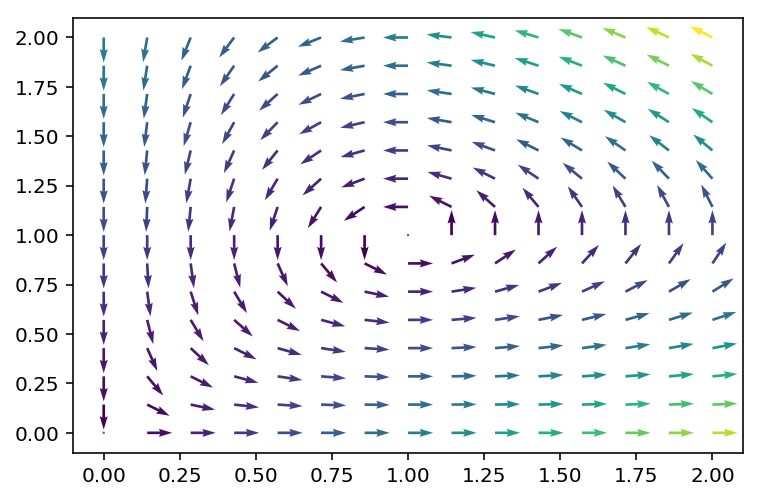
\includegraphics[width=0.8\columnwidth]{figures/lotka-volterra-direction-field.png}

  \caption{Direction field for the Lotka-Volterra model with $a = 0.5$ generated by a computer.}
\end{figure}

In the computer generated picture it is probably easier to tell what is
happening with the solutions. If one were to choose a point in the plane, a
solution going through that point would move in the direction of the vector in
that point. Repeating this process can give us a rough idea of what the
solutions look like: orbits around the stationary solution $(1,\ 1)$.


\subsection{Phase diagram of the Lotka-Volterra equations}

In our qualitative analysis of the Lotka-Volterra model we have found the
stationary solutions and more or less characterised the rest of the solutions
using the direction field. We would, however, like to have a more precise idea
of what the solutions look like. We will devote the rest of this section to
that.

\begin{dfn}
  [First integral]

  TODO. we really need a definition here :(
\end{dfn}


\section{Stability theory}

Consider the general autonomous system
\begin{align}
  \label{eq:autonomous-stability}
  \vec{x}' = f(\vec{x})
\end{align}
where $f: \Omega \subset \R^n \to \R^n,\ \Omega$ is open and $f \in
C^2(\Omega)$.

\begin{dfn}
  [Lyapunov stability] Let $\vec{x}^*$ be a stationary solution to
  \ref{eq:autonomous-stability}. We say $\vec{x}^*$ is Lyapunov stable (or just
  stable for short) if for every open neighbourhood $U$ of $\vec{x}^*$ there
  exists an open neighbourhood $V$ of $\vec{x}^*$ such that any solution
  $\vec{x}$ of \ref{eq:autonomous-stability} with $\vec{x}(0) \in B$ satisfies
  $\vec{x}(t) \in U$ for all $t > 0$.
\end{dfn}

\begin{dfn}
  [Asymptotic stability]

  Let $\vec{x}^*$ be a stationary solution to \ref{eq:autonomous-stability}. We
  say $\vec{x}^*$ is asymptotically stable if there exists an open
  neighbourhood $W$ of $\vec{x}^*$ such that for any solution $\vec{x}$ of
  \ref{eq:autonomous-stability} with $\vec{x}(0) \in W$ it holds that
  \[
    \norm{\vec{x}(t) - \vec{x}^*} \to 0 \text{ as } t \to \infty.
  \]
\end{dfn}

\begin{remark}
  If $\vec{x}^*$ is asymptotically stable then it is Lyapunov stable.
\end{remark}

\subsection{Linear stability analysis}

\begin{dfn}
  Let $\vec{x}^*$ be a stationary solution to \ref{eq:autonomous-stability}.
  The linear system
  \begin{align}
    \label{eq:linear-system-stability}
    \vec{y}' = Df(\vec{x}^*)\vec{y}
  \end{align}
  is called a linearisation of \ref{eq:autonomous-stability} in $\vec{x}^*$.

  Moreover, $\vec{x}^*$ is called linearly unstable, resp. stable /
  asymptotically stable if $\vec{0}$ is unstable, resp. stable / asymptotically
  stable for \label{eq:linear-system-stability}.
\end{dfn}

\begin{thm}
  [Principle of linearised stability]

  If $\vec{x}^*$ is linearly asymptotically stable, resp. unstable, then
  $\vec{x}^*$ is asymptotically stable, resp. unstable.
\end{thm}

\begin{remark}
  The previous theorem does not work for Lyapunov stability, i.e.
  \[
    \vec{x}^* \text{ linearly stable } \nRightarrow \vec{x}* \text{ stable}.
  \]
\end{remark}



  \chapter{Calculus of variations}

\begin{dfn}
  [Variational problem]

  Let $X$ be a real vector space (of functions, possibly infinite dimensional),
  $\calA \subset X$ a set of admisible functions and $\calI : X \to \R$ a
  functional that assigns a real number for each $u \in X$.

  A variational problem is the task
  \[
    \text{minimise } \calI(u),\quad u \in \calA.
  \]
\end{dfn}

In particular we are concerned with variational problems of integral form, i.e.
those where
\begin{align}
  \label{eq:cv-integral}
  \calI(u) = \int_a^b f(x, u(x), u'(x))dx,
\end{align}
where $u : [a, b] \to \R^m$ and $f: [a,b] \times \R^m \times \R^m \to \R$.

As mathematicians, we are immediately concerned about the exitence and
uniqueness of solutions. Until 1850, it was thought that minimisers for
integral problems always existed but Weierstrass gave a counter example. From
that moment on, a new theory for solving variational problems, now known as the
direct method was developed. In this section we will mostly concentrate on the
classical method for finding minimisers which basically replicates the process
of finding minima for functions in vector calculus. The reason for this is that
a formal treatment of the direct method requires advanced mathematical tools
from functional analysis, which is not a prerequisite for this course.

\section{The classical method}

This method was developed by Euler and Lagrange during the 18th century. The
strategy for dealing with variational problems of the form
\eqref{eq:cv-integral} is to just go ahead and find the minima of the function
$\calI(u)$. For this, let us recall the approach taken in vector calculus to minimise a function $f: \R^m \to \R^n$.
\begin{enumerate}
  \item Find $\overline{x} \in \R^m$ such that $Df(\overline{x}) = \0$,
  \item Find $D^2f(\overline{x})$, and
  \item Check that $D^2f(\overline{x})$ is positive definite.
\end{enumerate}

The problem with this strategy is that we don't know if $Df$ or $D^2f$ will
exist for our functional $f = \calI$. Therefore, we will introduce a weaker
notion of derivative, the variation, which is easier to work with in the
context of these problems.

\begin{dfn}
  [Admissible perturbation]

  Let $X$ and $\calA$ be a function space and a set of admissible functions,
  resp. Let $u \in \calA$. For any $\varphi \in X$ we say $\varphi$ is an
  admissible perturvation of $u$ iff there exists a $\varepsilon_0 > 0$ such
  that
  \[
    u + \varepsilon \varphi \in A,\quad \text{ for every } \varepsilon \in
    (-\varepsilon_0, \varepsilon_0).
  \]
\end{dfn}


\begin{dfn}
  [Variation]

  Let $X = \{ f : A \to B \}$ be a function space, $u, \varphi \in X$ and $x
  \in A$. We define the variation of $u$ at $a$ in the direction of $\varphi$
  as
  \begin{align}
    \label{eq:variation}
    \delta u(a)(\varphi) = \left. \frac{d}{d\varepsilon}\right|_{\varepsilon =
    0} u(a + \varepsilon \phi).
  \end{align}
\end{dfn}


\section{Exercises}

\begin{ex}
  [Dido's problem]

  Let $L > 0$ be a given length. We consider the maximisation problem
  \[
    \text{maximise } \int_0^L u(s)\sqrt{1 - u'(s)^2}ds, \text{ for } u \in \calA,
  \]
  where $\calA = \{C^1((0, L)) \cap C^0([0, L]) : u(0) = 0, u(L) = 0,
  \abs{u'(s)} \text{ for } s \in (0, L)\}$, which emerges from modeling Dido's
  problem.

  \begin{enumerate}
    \item Determine the corresponding Euler-Lagrange equation and find a
      non-negative solution $\overline{u} \in \calA \cap C^2((0, L))$.
    \item Sketch the curve $\{(\varphi(s), \overline{u}(s)) : s \in [0, L]\}$
      with $\varphi(s) = \int_0^s \sqrt{1 - \overline{u}'(\tau)}d\tau$ for $s
      \in [0, L]$.
    \item Interpret b) in the context of Dido's problem.
  \end{enumerate}

  \textit{Hint for a):} \footnote{In the original statement for this problem,
  the hint was only a simple implication, but by proving it one realised that
it was a double implication.}Prove and use the following statement: Let $a, b
\in \R$ with $a < b,\ u \in C^2((a, b))$ and $f \in C^2(\R \times \R)$ such
that $\partial_p f(u, u') \in C^1(a, b)$. Then
  \[
    \ddx \partial_p f(u, u') = \partial_z f(u, u')\text{ in } (a, b)
  \]
  if, and only if, there exists $c \in \R$ such that
  \[
    f(u, u') - u' \partial_p f(u, u') = c\text{ in } (a, b).
  \]
\end{ex}

\begin{proof}
  [Proof of the hint]
  Not very precise but something along the lines of
  \begin{align*}
         & \ddx \partial_p f(u, u') = \partial_z f(u, u') \\
    \iff & \partial_z f(u, u') - \ddx \partial_p f(u, u') = 0 \\
    \iff & \int \partial_z f(u, u') - \int \ddx \partial_p f(u, u') = \int 0 \\
    \iff & f(u, u') - u' \partial_p f(u, u') = c.
  \end{align*}

  Or, with derivatives,
  \begin{align*}
    & f(u, u') - u'\partial_p f(u, u') = c \\
    \iff & \ddx f(u, u') - \ddx u' \partial_p f(u, u') = \ddx c \\
    \iff & \partial_z f(u, u') u' + \partial_p f(u, u')u'' - u'' \partial_z f(u, u') - u' \ddx \partial_p f(u, u') = 0 \\
    \iff &u' \left( \partial_z f(u, u') - \ddx \partial_p f(u, u')\right) = 0.
  \end{align*}
  In this case, if $u' \neq 0$ we have
  \[
  \partial_z f(u, u') - \ddx \partial_p f(u, u') = 0 \iff
  \ddx \partial_p f(u, u') = \partial_z f(u, u').
  \]
  Otherwise, we go back to the original equation
  \[
    f(u, u') - 0 \partial_p f(u, u') = c \iff  f(u, u') = c
  \]
  which means that $f$ is constant in $u$ and therefore in $x$ so it is trivial to see that
  \[
    \partial_p f(u, u') = 0 = \partial_z f(u, u'),
  \]
  which gives the first equation.
\end{proof}


\begin{proof}
  For the purposes of determining the Euler-Lagrange equation we have $x = s,\
  z = u(x),\ p = u'(s)$ and $f(x, z, p) = z\sqrt{1 - p^2}$. The involved
  partial derivatives are
  \[
    \partial_z f(x, z, p) = \sqrt{1 - p^2} \text{ and }
    \partial_p f(x, z, p) = - \frac{zp}{\sqrt{1 - p^2}},
  \]
  and thus the Euler-Lagrange equation becomes
  \[
    \ddx \frac{- u u'}{\sqrt{1 - u'^2}} = \sqrt{1 - u'^2}.
  \]
  This looks complicated so we apply the hint:
  \begin{align*}
    & u\sqrt{1 - u'^2} + u' \frac{uu'}{\sqrt{1 - u'^2}} = c \\
    \iff & u \left( \sqrt{1 - u'^2} + \frac{u'^2}{\sqrt{1 - u'^2}}\right) = c \\
    \iff & u \left( \frac{1 - u'^2 + u'^2}{\sqrt{1 - u'^2}}\right) = c \\
    \iff & u = c\sqrt{1 - u'^2} \\
    \iff & u' = \sqrt{1 - \left( \frac{u}{c} \right)^2}.
  \end{align*}
  That last equation desperately screams for separation of variables and a trigonometric change of variable:
  \begin{align*}
    & \frac{du}{ds} = \sqrt{1 - \left( \frac{u}{c} \right)^2} \\
    \iff &\frac{du}{\sqrt{1 - (u/c)^2}} = ds \\
    \iff & \int \frac{1}{\sqrt{1 - (u/c)^2}} du = \int ds.
  \end{align*}
  Change $u / c = \sin y \implies u = c\sin y \implies du = c\cos y dy$ to get
  \begin{align*}
    \int \frac{1}{\sqrt{1 - (u/c)^2}} du
  & = \int \frac{1}{1 - \sin^2 y} c \cos y dy \\
  &= c \int \frac{\cos y}{\cos y} dy = cy \\
  &= c\arcsin\frac{u}{c}
  \end{align*}
  Plugging it back into the hint,
  \[
    s + k = c\arcsin\frac{u}{c} \implies u(s) = c\sin \frac{k+s}{c},
  \]
  which we rewrite picking different constants,
  \[
    u(s) = k_1 \sin( k_2 s + k_3),
  \]
  where the constants $k_1, k_2, k_3$ are obtained by enforcing $u \in \calA$.
  More specifically, we require
  \[
    u(0) = 0 \implies k_3 = 0\text{ and } u(L) = 0 \implies k_2 L = n\pi.
  \]
  Moreover, we require $u$ to be non-negative, therefore $n = 1$ and thus $k_2
  = \frac{\pi}{L}$ (otherwise the sine would go negative). Finally, we want
  \[
    \abs{u'(s)} < 1 \implies \abs{k_1\cos(k_2s + k_3) k_2} < 1
    \implies k_1 k_2 < 1 \implies k_1 < \frac{L}{\pi},
  \]
  since we require that $k_1$ is positive so that $u(s)$ also is. This final
  parameter is fixed by maximising $\calI(u)$:

  TODO
\end{proof}


\begin{ex}
  [Geodesics in $\R^2$]

  Let $A$ and $B$ be two points in the plane. What is the shortest connection between $A$ and $B$?

  \begin{enumerate}
    \item Set up the variational problem to model the situation.
    \item Solve the problem and interpret the result.
  \end{enumerate}
\end{ex}

\begin{proof}
  Let $X = C^1([0,1]; \R^2)$ and $\calA = \{ u \in X \mid u(0) = A,\ u(1) =
  B\}$. We define our functional $\calI$ as the length of the parametrised
  curve $u$ as follows
  \[
    \calI(u) = \int_0^1 \norm{u'(t)} dt.
  \]
  Our variational problem is
  \[
    \text{minimise } \calI(u) \text{ for } u \in \calA.
  \]

  To solve it we use the Euler-Langrange method. We have $f(t, u(t), u'(t) =
  \norm{u'(t)}$ and, in the form of the Euler-Langrange equations, we get $f(x,
  z, p) = \norm{p}$. Therefore,
  \[
    \delta_z f = 
    \begin{pmatrix}
      0 & 0
    \end{pmatrix}
    \text{ and } \delta_p f =
    \begin{pmatrix}
      \frac{p_1}{\norm{p}} & \frac{p_2}{\norm{p}}
    \end{pmatrix}.
  \]
  Notice how $p = u' : [0, 1] \to \R^2$ so by $\delta_p f$ we really mean the
  last two numbers in $Df$ (which is a row matrix since $f$ is real valued). We
  arrive at the following Euler-Lagrange equation
  \[
    \ddt \delta_p f = \delta_z \iff \ddt
    \begin{pmatrix}
      \frac{u_1}{\norm{u}} & \frac{u_2}{\norm{u}} 
    \end{pmatrix}
    =
    \begin{pmatrix}
      0 & 0
    \end{pmatrix}.
  \]
  Instead of taking the derivative with respect to $t$, we may simply rewrite
  this as
  \[
  \begin{pmatrix}
    \frac{u_1}{\norm{u}} & \frac{u_2}{\norm{u}}
  \end{pmatrix}
  =
  \begin{pmatrix}
    c_1 & c_2
  \end{pmatrix},
  \]
  where $c_1, c_2 \in \R$ are constants.

  Therefore
  \[
    u(t) = \int u'(t) dt = (c_1 t, c_2 t) + u_0,\ u_0 \in \R^2,
  \]
  which is a parametrisation for a curve. The parameters $c_1, c_2$ and $u_0$
  are determined by enforcing $u \in \calA$:
  \[
    u(0) = u_0 = A,\ u(1) = (c_1, c_2)  + u_0 = B.
  \]
\end{proof}

  \chapter{Continuum mechanics}

This chapter deals with the physics of a very general body that we describe
using calculus, hence the name continuum. The main assumption that we make to
be able to do this is that the behaviour of a system can be described by
averaging some characteristic quantities over the space it occupies, instead of
computing every one of them for every atom or molecule, i.e. that the involved
quantities in a problem are defined in a continuum. It turns out this
assumption is pretty good and the models we will get closely describe what is
happening in reality.

\section{Frames of reference and coordinate systems}

Before we begin we need a way to describe points in space. We will do this
using the standard definitions and results of affine spaces that we get from
linear algebra.

\begin{dfn}
  Let $\{e_1, \dots, e_n\}$ be an orthonormal basis for $R^n$ and let $O \in
  \R^n$ be a point which we will call the origin. In the equation
  \[
    X = O + \sum_{i = 1}^n x_i e_i,
  \]
  we define $(x_1, \dots, x_n)$ to be the coordinates of the point $X$ with
  respect to the origin $O$.
\end{dfn}

Notice how in the above definition we talked about points and not vectors when
dealing with $X$ and $O$. The distinction is rather technical and can almost
always be ignored but in short the deal is that points live in the affine space
$\mathbb{A}^n_\R = (A, \R^n, f)$ while vectors live in $\R^n$. An affine space
always comes with a function that maps points to vectors and is generally of
the form
\[
  f : A \times A \to \R^n,\qquad (P, Q) \mapsto \overrightarrow{PQ},
\]
where $\overrightarrow{PQ}$ denotes the vector which starts at $P$ and ends at
$Q$ that can be computed by treating $P$ and $Q$ as vectors in $\R^n$ and
taking the difference. More details can be found in \cite{wikiaffine}.


One important takeaway is the following lemma.

\begin{lem}
  Let $(O; e_1, \dots, e_n)$ and $(O^*, e_1^*, \dots, e_n^*)$ be two affine
  coordinate systems and let $X$ be a point in $\mathbb{A}^n_\R$ defined in the
  two coordinate systems, i.e.
  \[
    X = O + \sum_{i = 1}^n x_i e_i = O^* + \sum_{i = 1}^n x_i^* e_i^*,
  \]
  then there exists $a \in \R^n$ and $Q \in \R^{n\times n}$ orthogonal such that
  \[
    x^* = a  + Q x.
  \]
\end{lem}


\section{Introduction and setup of continuum mechanics}

\subsection{Lagrangian and Eulerian coordinate systems}

Some of the problems we will focus on require us to describe the evolution of
the shape of a body. We might do this by following the position of a point
inside the body as time passes. To be precise, we choose an initial state or
\textbf{reference configuration} $\Omega \subset \R^n$, which is normally the
set of all points in space which are part of the body under consideration. Lets
say that \textbf{material point} is called $X \in \Omega$. We can think of $X$
as a way to pinpoint an atom in the body and lets assume that we can track it
as time passes. We might describe its position with the function
\[
  x : \R \times \R^n \to \R^n,\qquad (t, X) \mapsto x(t, X).
\]

On the other hand, we may be interested in some other quantities, for instance
the temperature at a point in the body. While it could be the case that we are
interested in the temperature of a particular atom (even if that made sense), it
is most likely that we are looking for the evolution of temperature at a fixed
point in space. It could even be that we are dealing with a fluid and looking
at individual atoms or molecules does not make sense. In both of this cases we
are interested in a quantity $\varphi(t, x)$ where $x \in \R^n$. The choice of
the letter $x$ for the physical point is not a coincidence since for a material
point $X$ in the reference configuration we can get its position at time  $t$
with $x(t, X)$ and therefore $\varphi(t, x) = \varphi(t, x(t, X))$.

Let us formalise these concepts. We start by making suitable assumptions
\begin{enumerate}
  \item The material point $X$ is described by its position at some initial
    time $t = t_0$ by the function $X = x(t_0, X)$.
  \item The mapping $(t, X) \mapsto x(t, X)$ is continuously differentiable.
  \item For all $t \geq t_0$, the mapping $x$ is invertible.
  \item $x$ is orientation preserving, i.e. the matrix\footnote{The book
      \cite[p. 207]{eck2017mathematical} calls the determinant of this matrix
      the Jacobi determinant. In reality, $Jx$ is just the the differential
      matrix $Dx$ only we omit the first row since we are interested in the
      derivatives with respect to the coordinates of the material point $X$.
      Notice how we say differential matrix since the Jacobian matrix is
      guaranteed to exist and be the derivative because we asked for $x$ to be
      continuously differentiable.}
    \[
      Jx(t, X)_{ij} = \left( \frac{\partial x_i}{\partial X_j} (t, X) \right)
    \]
    has a positive determinant for every $t \geq t_0$ and every $X \in \Omega$.
\end{enumerate}

The terms $x$ and $X$ represent two different types of coordinates\footnote{I
tried to phrase this first part of the section as a standard
definition-properties introductory section. However, these constructs are
sometimes just notational conventions used by people who work with different
branches of continuum mechanics and hence are not normally that clearly
defined. One may take this section with a grain of salt and just make sure the
math makes sense when dealing with equations on each coordinate system.}
corresponding to the two ways of looking at a problem described before:
\begin{itemize}
  \item \textbf{Lagrangian coordinates} $X$ allow us to choose one material point and
    follow its evolution, while
  \item \textbf{Eulerian coordinates} $x$ relate to a fixed point in space.
\end{itemize}

In general, we will observe different material points at different times at
point $x$ specified in Eulerian coordinates.

\subsection{Analysis of relevant quantities in Lagrangian and Eulerian coordinate systems}

Before we move on, let's take a moment to really formalise how the function $x$
is defined and to look at how we might take the derivatives. In the book
(\cite[p. 208]{eck2017mathematical}) we can find the following definition

\begin{dfn}
  [Material time derivative]

  Let $\varphi : \R \times \R^3 \to \R$. We define the material time derivative
  of $\varphi$ with respect to $t$ as
  \[
    D_t\varphi(t, x) = \partial_t \varphi(t, x) + \nabla \varphi(t, x) \cdot v(t, x),
  \]
  where $v(t, x) = \partial_t x(t, X(t, x))$.
\end{dfn}

To me, this did not make sense at all on the first reading. It also didn't make
sense on the second, third, and $n$-th readings, for a substantially large $n$.
What helped me understand it was to not take it as a definition, but to try to
arrive at the same result with standard vector calculus results, i.e. the chain
rule. In what follows I try to describe this to the best of my ability.

Take any $X_0 \in \Omega$ and define $x_0(t) = x(t, X_0)$, i.e. fix the second
parameter of the function $x(t, X)$ so that it describes the position of only
one particular material point $X_0$. In this case,
\[
  \ddt x_0(t) = \left. \partial_t x(t, X)\right|_{X = X_0}.
\]
Now going back to our relevant quantity $\varphi$ we do the same
thing---restrict it to work for just one material point $X_0$. In this case
$\varphi$ becomes $\varphi(t, x_0(t))$.







We will use the convention that quantities expressed as a function of
Lagrangian coordinates will be denoted by [greek] capital letters like $\Phi(t,
X)$ while quantities defined on Eulerian coordinates will be identified by a
lowercase letter $\varphi(t, x(t, X))$. It is important to observe that here
\[
  \Phi(t, X) = \varphi(t, x(t, X)),
\]
that is, they denote the same quantity and hence evaluate to the same
mathematical object (in some cases we use vectors or matrices instead of just
numbers to represent relevant quantities).

One instance where this convention is used is when dealing with the velocity
fields, which are
\[
  V(t, X) = \frac{\partial x}{\partial t}(t, X)
\]
in Lagrangian coordinates, and
\[
  v(t, x) = V(t, X(t, x))
\]
in Eulerian coordinates. Here $X$ is the inverse of the function $x$ which we
assumed to exist for $t \geq t_0$.

More generally, we may wish to calculate the derivative of a quantity. In
Eulerian coordinates, when we denote a quantity by $\varphi(t, x)$ we must not
forget the fact that $x$ is itself a function of $t$ and a material point $X$.
More explicitly, we may write $\varphi(t, x(t, X))$ as before to make it easier
to compute the derivative with respect to time using the chain rule.


We conclude this section by defining two sets of important curves, namely
pathlines and streamlines.

\begin{dfn}
  [Pathlines]

  Pathlines are solutions of the equation
  \[
    y'(t) = v(t, y(t)).
  \]
\end{dfn}

They describe the paths followed by a material point during the evolution of
the system.

\begin{dfn}
  [Streamlines]

  Streamlines are solutions to the equation
  \[
    z'(s) = v(t, z(s)).
  \]
\end{dfn}

They are curves tangent to the velocity field at every point, i.e. they give a
\textit{snapshot} of the velocity field at time $t$.

Observe that in streamlines we treat $t$ as a parameter whereas the equation
for pathlines is more involved. See the solution TODO add reference to extra problem.


Throughout the next sections, the structure will be the following. We will
first focus on fluids and for that we will use Eulerian coordinates.  This will
take the greater part of the chapter. Finally, we will conclude with elastic
solids, for which we will use Lagrangian coordinates.

\section{Reynold's transport theorem}

We start with some basic results from calculus / algebra.

\begin{lem}
  [Jacobi's formula]
  Let $t \mapsto A(t) \in \R^{n \times n}$ be a differentiable map such that
  $A(t)$ is invertible. Then,
  \[
    \ddt \det A(t) = \tr \left( \inv{A}(t) \ddt A(t) \right) \det A(t).
  \]
\end{lem}

This result can be proved by setting $\det A = F(a_{11}, \dots, a_{nn})$ as a
function of the entries of the matrix $A$ and appyling the cain rule with a lot
of care. See TODO for details.

\begin{thm}
  Let $(t, X) \mapsto x(t, X)$ be a continuously differentiable, invertible and
  orientation preserving mapping, and that $(t, X) \mapsto \partial_t x(t, X)$
  is also continuously differentiable. Then,
  \[
    \partial_t J(t, X) = \left. \nabla \cdot v(t, x)\right|_{x = x(t, X)} J(t, X),
  \]
  where $J$ is the matrix introduced in the previous section.
\end{thm}

  \chapter{Partial differential equations}

Unlike with ODEs, there is no general theorem for existence, uniqueness or
structure of solutions for PDEs. In this section we will classify some of the
most common PDEs and try to give some results for each category that help solve
them or gain some insight on how the solutions behave.

\begin{dfn}
  A partial differential equation or PDE is an identity of the form
  \begin{equation}
    \label{eq:pde}
    F(D^k, \dots, D^2, \nabla u, u, x) = 0
  \end{equation}
  where
  \begin{itemize}
    \item $x \in \Omega \subset \R^n$ is the independent variable,
    \item $u : \Omega \subset \R^n \to \R$ is the function we want to solve
      \eqref{eq:pde} for,
    \item TODO
  \end{itemize}

  TODO: comment about the order
\end{dfn}


\section{First-order partial differential equations}

In general, first-order PDEs can be linear, semilinear, quasilinear or
non-linear. An example of a non-linear equation is the TODO eq
\[
  \norm{\nabla u(x)} = 1.
\]
An example of a linear equation is the generic transport equation
\[
  \partial_t u(t, x) + \partial_x u(t, x) = 0.
\]

In general all but non-linear equations can be solved using the so called
\textbf{method of characteristics} which exploits certain geometric properties
to reduce the PDE to a system of ODEs.

\subsection{Method of characteristics for linear partial differential equations}

\section{Second-order partial differential equations}

In this harder case, we will restrict ourselves to just linear equations.

\begin{dfn}
  [Second-order, linear PDE]

  We say the identity
  \begin{equation}
    \label{eq:semilinear-2o}
    \sum_{j, k = 1}^n a_{jk}(x) \partial_{x_j} \partial_{x_k} u(x)
    + F(\nabla u(x), u(x), x) = 0
  \end{equation}
  with
  \[
    A(x) = \left( a_{jk}(x) \right)_{j, k = 1}^n \in \R^{n \times n} \text{ symmetric}
  \]
  is a linear second-order partial differential equation.
\end{dfn}

Note that the symmetricness of the matrix $A(x)$ comes from Schwarz's theorem
for mixed derivatives.

\begin{dfn}
  Consider a semilinear second-order PDE of the form of
  \eqref{eq:semilinear-2o}. For any $x \in \Omega$ we say
  \eqref{eq:semilinear-2o} is
  \begin{itemize}
    \item \textbf{elliptic} at $x$ if all the eigenvalues of $A(x)$ are
      non-zero and have the same sign,
    \item \textbf{parabolic} at $x$ if $A(x)$ has the eigenvalue 0 with
      multiplicity one and all other eigenvalues have the same sign, and
    \item \textbf{hyperbolic} at $x$ if 0 is not an eigenvalue of $A(x)$ and
      exactly $n - 1$ eigenvalues have the same sign.
  \end{itemize}

  If any of the previous contitions holds for every $x \in \Omega$ we say
  \eqref{eq:semilinear-2o} is \textbf{globally} elliptic, resp. parabolic,
  hyperbolic.
\end{dfn}

\begin{eg}
  The Laplace equation $\Delta u(x) = 0$ is globally elliptic since
  \[
    \Delta u(x) = \sum_{i = 1}^n \partial^2_{x_i} u(x)
    = \sum_{i = 1}^n 1 \partial_{x_i} \partial_{x_i} u(x)
    \implies A(x) = \Id.
  \]
\end{eg}

\begin{eg}
  The heat equation $\partial_t u(t, x) - \Delta u(t, x) = 0$ is globally
  parabolic since
  \[
    A(x) =
    \left(
      \begin{array}{c|ccc}
        0 & 0 & \dots & 0 \\ \hline
        0 & -1 & \dots & 0 \\
        0 & 0 & \ddots & 0 \\
        0 & 0 & \dots & -1
      \end{array}
    \right).
  \]
\end{eg}

\begin{eg}
  The wave equation $\partial^2_t u(t, x) - \Delta u(t, x) = 0$ is globally
  hyperbolic since
  \[
    A(x) =
    \left(
      \begin{array}{c|ccc}
        1 & 0 & \dots & 0 \\ \hline
        0 & -1 & \dots & 0 \\
        0 & 0 & \ddots & 0 \\
        0 & 0 & \dots & -1
      \end{array}
    \right).
  \]
\end{eg}

\subsection{Results for elliptic second-order partial differential equations}

Since the elliptic is the simplest of the three categories, we will use the
remaining time to give some results about two very important examples of these
equations: the Laplace equation and the Poisson equation.

\subsubsection{Fundamental solution to the Laplace equation}

Recall that the Laplace equation is of the form
\begin{equation}
  \label{eq:pde-laplace}
  \Delta u(x) = 0
\end{equation}
for some $u$ TODO.

We make the ansatz $u(x) = w(\norm{x}) = w(r)$, i.e. we assume rotational
symmetry of the solution. If this were the case then \eqref{eq:pde-laplace} becomes
\[
\Delta u
\]

\begin{dfn}
  [Convolution product]

  Given two functions $f, g : \Omega \subset \R^n \to \R$ we define the
  convolution product of $f$ and $g$ as
  \[
    (f \ast g)(x) = \int_\Omega f(x - y) g(y) dy.
  \]
\end{dfn}

That we name this weird thing product is not coincidental, as it shares some
properties with the standard number product.

\begin{thm}
  [Properties of the convolution product]
   Let $f, g : \Omega \subset \R^n \to \R$ be two functions. Then
   \begin{enumerate}
     \item (Conmutativity) $f \ast g = g \ast f$, and
     \item (Linearity with respect to differentiation)
       \[
         \partial_{x_j}^k (f \ast g)
         = (\partial_{x_j}^k f) \ast g
         = f \ast ( \partial_{x_j}^k g).
       \]
   \end{enumerate}
\end{thm}

We will finish the course with two results about vector valued functions.

\begin{thm}
  Let $\Omega \subset \R^n$ and let $B_R(x) \subset \Omega$ be a ball with
  radius $R > 0$ centered in $x \in \Omega$. If $u \in C^2(\Omega)$ is harmonic
  then
  \[
    u(x)
    = \frac{1}{\norm{\partial B_R(x)}} \int_{\partial B_R(x)} u(y) d s_y
    = \frac{1}{\norm{B_R(x)}} \int_{B_R(x)} u(y) dy,
  \]
  where $\norm{\partial B_R(x)}$ denotes the hypersurface area of the boundary
  of $B_R(x)$ and $\norm{B_R(x)}$ denotes the hypervolume of the ball $B_R(x)$.
\end{thm}

Note that in the previous theorem we have not inlined the well known formulas
for the area and volume of a sphere as these only hold for $R^3$.


TODO: other theorem or maximum principle.





	
	
	% \listoftheorems[ignore={dfn,ex,eg,remark,lem,cor}]
	
	\bibliographystyle{IEEEtran}
	\bibliography{IEEEabrv,mm-notes}
\end{document}